\fancyhead{}
\fancyfoot{}
\newtheorem{teorema}{Teorema}
\cfoot{\thepage}

\lhead{Conceptos fundamentales, teorías y antecedentes}
%\rhead{\today}
%\rfoot{\thepage}

\chapter{Conceptos fundamentales, teorías y antecedentes}

\section{Predicciones de Compras}

La predicción es el proceso de anticipar la cantidad y tipo de insumos que un negocio gastronómico necesitará adquirir en el futuro, con el objetivo de asegurar un suministro adecuado y eficiente.


\subsection{Relación de Demanda y Gestión de Suministro}

La relación de demanda y gestión de suministro se refiere a la interacción entre la cantidad de productos o insumos que los clientes requieren (demanda) y cómo la empresa se asegura de tener suficientes suministros disponibles para satisfacer esa demanda de manera eficiente. En un negocio gastronómico, la gestión de suministros es crucial para evitar situaciones en las que falten ingredientes clave, lo que podría afectar negativamente la calidad del servicio y la satisfacción del cliente.


\subsection{Importancia de la Predicción de Compra de Insumos}

La mayoría de las empresas distribuidoras de productos sufren de manera recurrente al no conocer la cantidad o un aproximado de productos que debería mantener en stock ya que, por un lado, si el stock es demasiado grande se pueden producir pérdidas de mercancía y costos innecesarios de transporte y almacenamiento, por el contrario, si el stock es demasiado pequeño, este será insuficiente para cubrir la demanda de los diferentes productos y se verá reflejado en la pérdida de clientes\cite{romero2021prediccion}. 

\vspace{1\baselineskip}
La aplicación de un modelo de predicción para planificar la demanda futura es un proceso circular de mejora continua. Eso significa que el modelo es enriquecido constantemente con datos en tiempo real para realizar predicciones más precisas y generar una planificación más acorde a la realidad \cite{decide}.
\begin{figure}[H]
  \begin{center}
    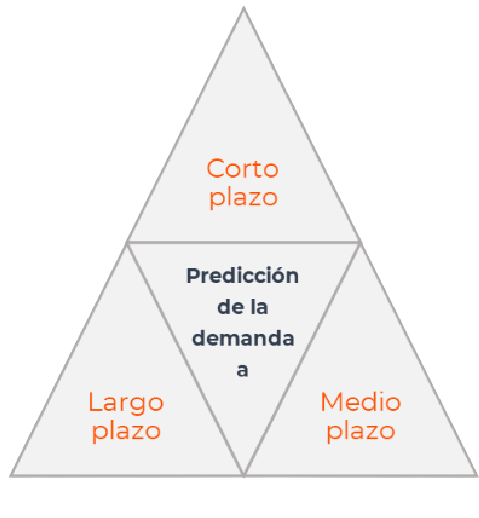
\includegraphics[scale=0.50]{./trianguloCMD.png}
    \caption{Predicción de demanda a corto, mediano y largo plazo\cite{decide}.}
    \label{fig:proceso_inventario}
  \end{center}
\end{figure}

\begin{enumerate}
  \item Utiliza la \textbf{Predicción de la demanda a largo plazo para la planificación estrategica.}
  Simula y compara diferentes escenarios hipotéticos de demanda, anticipate los cambios de mercado y planifica la contratación futura de recursos.
  \item Utiliza la \textbf{Predicción de la demanda a corto plaxo para la planificación operativa.}
  Planifica semanalmente las operaciones y recursos del día.
  \item Utiliza la\textbf{Predicción de la demanda a medio plazo para la planificación táctica.} 
  Conoce las capacidades con meses de antelacion y compáralas con las actuales para detectar posibles necesidades.
\end{enumerate}
\vspace{1\baselineskip}
La predicción de compra de insumos es vital para la planificación a corto, mediano y largo plazo en un negocio gastronómico por varias razones:



\begin{enumerate}
  \item \textbf{Optimización de Inventario:} El inventario tiene como propósito fundamental proveer a la empresa de materiales necesarios, para  su  continuo  y  regular  desenvolvimiento,  es  decir,  el  inventario  tiene  un  papel  vital  para  el funcionamiento acorde y coherente dentro del proceso de producción y de esta forma afrontar la demanda\cite{marques2017nivel}.
  
  Al prever la demanda futura, el negocio puede mantener un nivel de inventario óptimo. Comprar en exceso puede llevar al desperdicio de alimentos, mientras que comprar muy poco puede resultar en escasez y pérdida de ventas.

  \begin{figure}[H]
    \begin{center}
      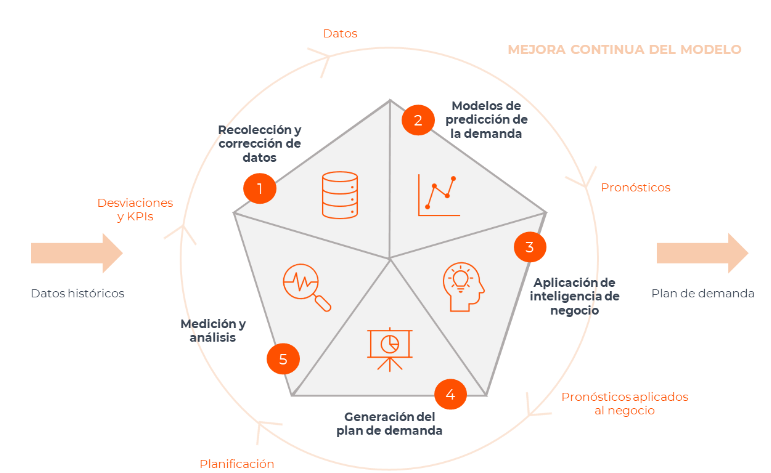
\includegraphics[scale=0.70]{./procesos_de_trabajo.png}
      \caption{Proceso de Optimización de inventario\cite{decide}.}
      \label{fig:proceso_inventario}
    \end{center}
  \end{figure}
  
  \item \textbf{Reducción de Costos:} Una predicción precisa permite comprar solo lo necesario, lo que reduce los costos asociados con el almacenamiento y la conservación de productos perecederos.
  
  Si  se  mantienen inventarios  demasiado  altos,  el  costo  podría  llevar  a  una  empresa  a  tener  problemas  de  liquidez financiera, esto ocurre porque un inventario “parado” inmoviliza recursos que podrían ser mejor utilizados en funciones más productivas de la organización\cite{marques2017nivel}.
  

  \item \textbf{Eficiencia Operativa:} Saber qué insumos se necesitarán en el futuro permite planificar y programar las operaciones de manera más eficiente, evitando retrasos y problemas logísticos.
  
  Es  útil  mantener  los  inventarios  en  las  empresas porque,  se  tiene  en  cuenta  la  capacidad  de  predicción  con  el  fin  de  planear  la  capacidad  y establecer un cronograma de producción, también fluctuaciones en la demanda ósea una reserva de  inventarios  a  la  mano  que  supone  protección,  inestabilidad  de  los  suministros,  protección  deprecios, descuentos por cantidad, menores costos de pedidos\cite{marques2017nivel}.

  
  
  \item \textbf{Satisfacción del Cliente:} Mantener un suministro constante de productos esencial para el negocio, ya que los clientes esperan encontrar su elección preferida en el menú en todo momento.
\end{enumerate}





\subsection{Factores que Influyen en la Curva de Insumos Demandados}

Varios factores pueden influir en el comportamiento de la curva de insumos demandados:

\begin{itemize}
    \item Día de la Semana y Estacionalidad: Los patrones de consumo pueden variar según el día de la semana y la temporada. Por ejemplo, los fines de semana pueden tener una mayor demanda en comparación con los días laborables.
    
    \item Eventos Especiales: Eventos como días festivos, celebraciones locales o conciertos cercanos pueden aumentar la demanda de alimentos y bebidas.
    
    \item Tendencias de Consumo: Las tendencias gastronómicas y las preferencias cambiantes de los consumidores pueden afectar la demanda de ciertos productos.
    
    \item Clima: Las condiciones climáticas también pueden influir en la demanda. Por ejemplo, un día caluroso podría aumentar la demanda de bebidas frías.
    
    \item Promociones y Ofertas: Las promociones especiales pueden aumentar temporalmente la demanda de ciertos productos.
\end{itemize}

\section{Sistema de información }

Según\cite{kendall2005analisis} el sistema de información\textit{ “Es un conjunto de elementos que interactúan entre sí, con el fin de apoyar las actividades de una empresa o negocio”}.

Es importante tener en cuenta que la necesidad de información en las organizaciones es vital para alcanzar el éxito y que un sistema de información debe justificar su implementación desde el punto de vista costo/beneficio, basándose en el valor que se le otorga a la información dentro de la organización \cite{kendall2005analisis}. Los beneficios pueden ser tangibles e intangibles, y dependen de los objetivos y necesidades de la organización.

Los sistemas de información se desarrollan para diferentes propósitos, según las necesidades de los usuarios humanos y la empresa. En definitiva, el uso adecuado de la información y la implementación de sistemas de información efectivos pueden marcar una gran diferencia en el éxito de una organización.

paragraph{ Tipos de sistema de información}

El propósito de un sistema de información, puede ser muy amplio, todo depende de las necesidades de la organización. Existen distintos tipos de sistemas de información, entre los que destacan los siguientes\cite{kendall2005analisis}:

\setcounter{secnumdepth}{3}
\paragraph{Sistemas de procesamiento de transacciones}

Se define como transacción un suceso que implica o afecta a una organización, y que está compuesta por datos referentes a ellas y que son de importancia para la organización\cite{kendall2005analisis}. Estos sistemas se encargan del procesamiento de los datos referentes a las transacciones, además de permitir la automatización de tareas y procesos operativos. 

La información que se obtiene como salida es utilizada posteriormente por los funcionarios de nivel operativo de la organización en la toma de decisiones. Las razones para el procesamiento de las transacciones son:  

\begin{itemize}
\item Clasificación: Implica agrupar todos los datos de acuerdo con características comunes.
\item Operaciones de cálculo: Consiste en realizar alguna operación para obtener resultados útiles.  
\item Ordenamiento: Consiste en disponerlos de alguna forma o secuencia, facilita el procesamiento y la búsqueda.  
\item Síntesis: Reduce los datos en información breve y concisa. 
\item Almacenamiento: Permite el registro de todas y cada una del suceso que afectan a la organización.

\end{itemize}

\paragraph{Sistema de información administrativa}

Los sistemas de información administrativa (MIS) no sustituyen a los sistemas de procesamiento de transacciones; más bien, todos los sistemas MIS incluyen el procesamiento de transacciones\cite{kendall2005analisis}. Los MIS son sistemas de información computarizados que funcionan debido a la decidida interacción entre las personas y las computadoras.

Al requerir que las personas, el software y el hardware funcionen en concierto, los sistemas de información administrativa brindan soporte a los usuarios para realizar un espectro más amplio de tareas organizacionales que los sistemas de procesamiento de transacciones, incluyendo los procesos de análisis y toma de decisiones. Para acceder a la información, los usuarios del sistema de información administrativa comparten una base de datos común; esta almacena tanto los datos como los modelos que permiten al usuario interactuar con ellos, interpretarlos y aplicarlos. Los sistemas de información administrativa producen información que se utiliza en el proceso de toma de decisiones. También pueden ayudar a integrar algunas de las funciones de información computarizadas de una empresa. 

\paragraph{Sistema de soporte de decisiones DSS}

Son sistemas de información que tienen como propósito auxiliar al usuario con las decisiones únicas que no se repiten y que no tienen una estructura definida\cite{kendall2005analisis}. Además de estar hechos a la medida de la persona o grupo que los usa en comparación con los Sistemas de información Gerencial. El propósito de estos sistemas es el de responder correctamente a condiciones inesperadas y propias de la información. Esto permite que sean empleados en niveles altos de la organización.  

\paragraph{Sistema de información gerencial}

Los Sistemas de Información Gerencial, también llamados Sistemas de Reportes de Gerencia, se dedican al apoyo de decisiones siempre que los requerimientos de información sean identificados, esto es, que la información que necesita para la toma de decisiones haya sido analizada anteriormente, y que esta misma decisión pueda tomarse nuevamente\cite{kendall2005analisis}. Estos sistemas pueden extraer la información necesaria de cualquier parte de la organización, por lo que la información necesaria ya se tiene almacenada al ser procesada por un sistema de transacciones. 


\paragraph{Sistema experto e inteligencia artificial }
La inteligencia artificial (IA) puede ser considerada como el campo dominante de los sistemas expertos. La idea general de la IA ha sido desarrollar equipos que se comporten de manera inteligente\cite{kendall2005analisis}. 

Dos ramas de investigación de la IA son: 

\begin{itemize}

\item La comprensión del lenguaje natural. 
\item El análisis de la habilidad para razonar un problema y llegar a una conclusión lógica. 

\end{itemize}

Los sistemas expertos utilizan las metodologías de razonamiento de la IA para resolver los problemas que los usuarios de negocios (y otros tipos de usuarios) les presentan. Los sistemas expertos son una clase muy especial de sistema de información que ha demostrado su utilidad comercial gracias a la disponibilidad extendida de hardware y software como las computadoras personales (PC) y las interfaces de sistemas expertos.


Un sistema experto (también conocido como sistema basado en el conocimiento) captura y utiliza en forma efectiva el conocimiento de uno o varios expertos humanos para resolver un problema específico al que una organización se enfrenta. Cabe mencionar que a diferencia de los sistemas DSS, que en última instancia dejan la decisión a la persona encargada de la toma de decisiones, un sistema experto selecciona la mejor solución para un problema o una clase específica de problemas. Los componentes básicos de un sistema experto son la base de conocimiento, un motor de inferencia que conecta al usuario con el sistema mediante el proceso de consultas en lenguajes, como el lenguaje de consulta estructurado (SQL), y la interfaz de usuario. Las personas conocidas como ingenieros del conocimiento capturan la experiencia de los expertos, crean un sistema computacional que incluye este conocimiento y después lo implementan\cite{kendall2005analisis}.



\begin{figure}[H]
  \begin{center}
    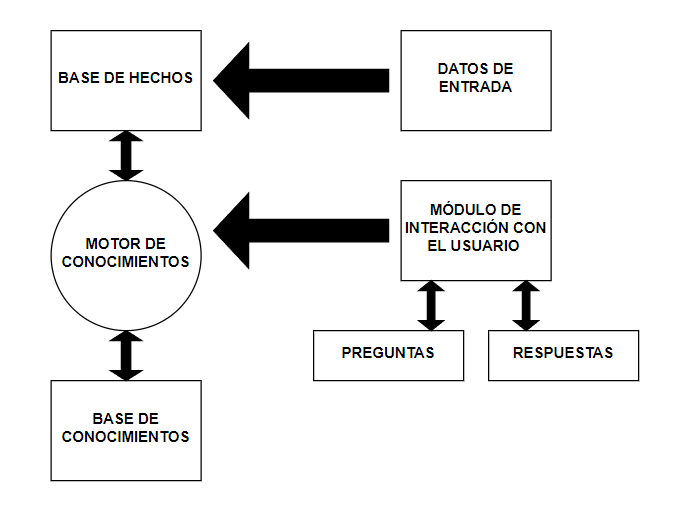
\includegraphics[scale=0.50]{./hechos.png}
    \caption{Arquitectura de un sistema experto \cite{diez2001introduccion}.}
    \label{fig:Arquitectura de un sistema experto}
  \end{center}
\end{figure}




En los Sistemas Expertos el conocimiento se hace explícito en forma de reglas, en la computación neuronal las ANN generan sus propias reglas aprendiendo de los ejemplos que se les muestran en la fase de entrenamiento\cite{olabe1998redes}. 



\section{Tiempos Actuales en las Predicciones de Demanda}

En la actualidad, las predicciones de demanda se benefician ampliamente de las tecnologías avanzadas y el análisis de datos. Las empresas pueden aprovechar sistemas de gestión de inventario y software de análisis de datos para recopilar y procesar información histórica y en tiempo real. Estas herramientas les permiten aplicar técnicas estadísticas y modelos de pronóstico para anticipar con mayor precisión los patrones de demanda futura.

En tiempos recientes, se ha observado la aplicación de diversas técnicas en el campo de la inteligencia artificial, como sistemas expertos, y más recientemente, algoritmos genéticos. Sin embargo, a pesar de esta evolución, los modelos que han captado una atención destacada son los basados en Redes Neuronales Artificiales (RNAs). Con el transcurso del tiempo, se han desarrollado múltiples arquitecturas de RNAs para abordar una variedad de problemas en el ámbito de la predicción de demanda.

\section{Mineria de datos}
La minería de datos puede definirse inicialmente como un proceso de descubrimiento de nuevas y significativas relaciones, patrones y tendencias al examinar grandes cantidades de datos\cite{perez2007mineria}.

El análisis de datos, potenciado por herramientas informáticas, ha dado lugar a la minería de datos. Esta disciplina busca descubrir automáticamente conocimiento en grandes bases de datos, identificando patrones, tendencias y perfiles a través de tecnologías avanzadas como el reconocimiento de patrones, redes neuronales y algoritmos genéticos.

Inicialmente, los sistemas de información se centraban en recopilar datos para apoyar la toma de decisiones. Con la informatización de las organizaciones, se amplió su función para respaldar los procesos esenciales. Ahora, se buscan prestaciones adicionales, como sistemas de información para la toma de decisiones.

La Minería de Datos se puede ubicar en el nivel más alto de la evolución de los procesos tecnológicos de análisis de datos \cite{martinez2001mineria}.

\section{El aprendizaje automático \textit{(machine learning)}}

\textit{Según Arthur Samuel, el aprendizaje automático se define como el campo de estudio que otorga a las computadoras la capacidad de aprender sin ser programadas explícitamente}\cite{mahesh2020machine}. 

El aprendizaje automático se utiliza para enseñar a las máquinas a manejar los datos de manera más eficiente. A veces, después de ver los datos, no podemos interpretar la información extraída de los mismos.En ese caso, aplicamos el aprendizaje automático.

Es decir, el aprendizaje automático como area de las ciencias computacionales aplicadas, desarrolla algoritmos capaces de tomar datos numéricos y alfanuméricos almacenados en un computador\cite{herrera2020prediccion}. 

Con la abundancia de conjuntos de datos disponibles, la demanda de aprendizaje automático está en aumento. Muchas industrias aplican el aprendizaje automático para extraer datos relevantes. El propósito del aprendizaje automático es aprender de los datos. Se han realizado muchos estudios sobre cómo hacer que las máquinas aprendan por sí mismas sin ser programadas explícitamente. Muchos matemáticos y programadores aplican varios enfoques para encontrar la solución a este problema que implica conjuntos de datos enormes\cite{mahesh2020machine}.

\vspace{1\baselineskip}
El Aprendizaje Automático se basa en diferentes algoritmos para resolver problemas de datos. A los científicos de datos les gusta señalar que no existe un único tipo de algoritmo que sea universal y mejor para resolver todos los problemas. El tipo de algoritmo utilizado depende del tipo de problema que se desee resolver, el número de variables, el tipo de modelo que se adapte mejor, entre otros factores. 

Las técnicas de machine learning son necesarias para mejorar la precisión de los modelos predictivos. Dependiendo de la naturaleza del problema empresarial que se está atendiendo, existen diferentes enfoques basados en el tipo y volumen de los datos\cite{ibm}.

En el contexto de la aplicación de algoritmos de Machine Learning en el cálculo de pronósticos de demanda, es esencial comprender que el objetivo principal de estos algoritmos es encontrar una función que tome un conjunto de variables como entrada y produzca una estimación del valor deseado, en este caso, la demanda. Esta función se ajusta a través del aprendizaje a partir de observaciones pasadas donde los datos de demanda son conocidos. Por ejemplo, utilizando datos de demanda de los últimos años, el modelo se entrena para desarrollar una función que pueda hacer predicciones precisas sobre la demanda futura, lo que implica una tarea de regresión, ya que el resultado esperado es un valor numérico real. Esta metodología se basa en el libro “Deep Learning” de Ian Goodfellow, Yoshua Bengio y Aaron Courville\cite{goodfellow2016deep}.

Una forma común de describir a un conjunto de datos u observaciones (dataset) es con una matriz de diseño. Una matriz de diseño es una matriz que contiene un ejemplo diferente en cada fila. Cada columna de la matriz corresponde a una característica diferente. Los algoritmos de aprendizaje se diferencian en función de la forma de operar y procesa los datos contenidos en una matriz de diseño\cite{arana2021redes}.

El siguiente diagrama muestra un flujo de trabajo típico para el uso del aprendizaje automático en modelado predictivo \cite{mirjalili2020python}:

\begin{figure}[H]
  \begin{center}
    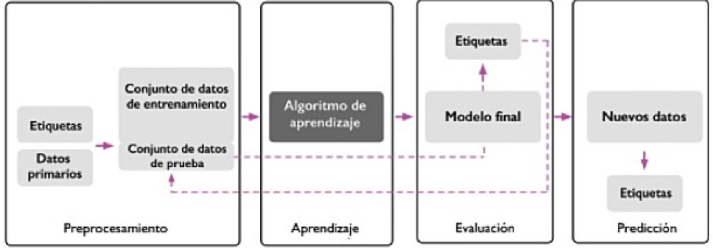
\includegraphics[scale=0.80]{./uso_aprendisaje_automatico.png}
    \caption{ flujo de trabajo típico para el uso del aprendizaje automático en modelado predictivo}
    \label{fig:perceptron}
  \end{center}
\end{figure}

\textbf{Procesamiento:}
  \begin{itemize}
    \item Extracción y escalado de características.
    \item Selección de características.
    \item Reducción de la dimensionalidad.
    \item Muestreo.
  \end{itemize}
\textbf{Aprendizaje:}%importante
  \begin{itemize}
    \item Selección del modelo.
    \item Validación cruzada.
    \item Medición del rendimiento.
    \item Optimización de hiperparametro.
  \end{itemize}

\section{Aprendizaje supervisado}

El aprendizaje supervisado comienza típicamente con un conjunto establecido de datos y una cierta comprensión de cómo se clasifican estos datos. El aprendizaje supervisado tiene la intención de encontrar patrones en datos que se pueden aplicar a un proceso de analítica. Estos datos tienen características etiquetadas que definen el significado de los datos. Por ejemplo, se puede crear una aplicación de machine learning con base en imágenes y descripciones escritas que distinga entre millones de animales\cite{ibm}.

\vspace{1\baselineskip}
El objetivo principal del aprendizaje supervisado es aprender un modelo, a partir de datos de entrenamiento etiquetados, que nos permite hacer predicciones sobre datos futuros o no vistos \cite{mirjalili2020python}. Aquí, el término supervisado se refiere a un conjunto de muestras donde las señales
de salida deseadas (etiquetas) ya se conocen.

\begin{figure}[H]
  \begin{center}
    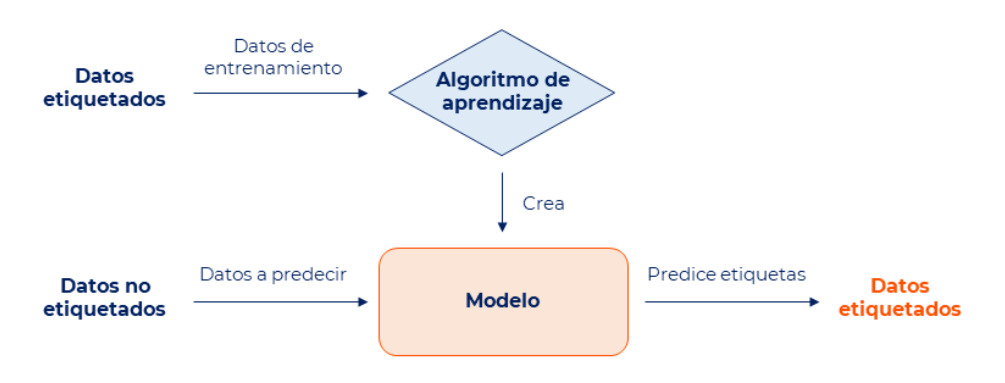
\includegraphics[scale=0.60]{./aprendisaje_supervisado.png}
    \caption{Aprendisaje supervisado\cite{decide}.}
    \label{fig:aprendisajesupervisado}
  \end{center}
\end{figure}

\section{Aprendizaje no supervisado}

El aprendizaje no supervisado se utiliza cuando el problema requiere una cantidad masiva de datos sin etiquetar. Por ejemplo, las aplicaciones de redes sociales, tales como Twitter, Instagram y Snapchat, tienen grandes cantidades de datos sin etiquetar. La comprensión del significado detrás de estos datos requiere algoritmos que clasifican los datos con base en los patrones o clústeres que encuentra. El aprendizaje no supervisado lleva a cabo un proceso iterativo, analizando los datos sin intervención humana\cite{ibm}.

Los métodos de aprendizaje no supervisados son utilizados durante el preprocesamiento de los datos antes de ser utilizados por algoritmos de característica supervisada. Estos algoritmos también son muy utilizados en la compresión de datos. Todos los métodos son implícita o explícitamente basados en la distribución de probabilidad en el espacio definido por las variables de entrada\cite{de2014aprendizaje}.

\section{Aprendizaje de refuerzo}

El aprendizaje de refuerzo es un modelo de aprendizaje conductual. El algoritmo recibe retroalimentación del análisis de datos, conduciendo el usuario hacia el mejor resultado. El aprendizaje de refuerzo difiere de otros tipos de aprendizaje supervisado, porque el sistema no está entrenado con el conjunto de datos de ejemplo. Más bien, el sistema aprende a través de la prueba y el error. Por lo tanto, una secuencia de decisiones exitosas conduce al fortalecimiento del proceso, porque es el que resuelve el problema de manera más efectiva \cite{ibm}.

\section{Redes Neuronales Artificiales}
Las Redes Neuronales Artificiales (RNA) son un componente esencial de la Inteligencia Artificial que emula el funcionamiento de las neuronas biológicas. Estas redes, entrenadas con entradas de escenarios internos o externos multiplicadas por pesos aleatorios, destacan en la resolución de funciones altamente no lineales, lo que las convierte en herramientas poderosas para la predicción. Inspiradas en el sistema nervioso biológico, encuentran aplicaciones en áreas como neurociencias, matemáticas, estadísticas y más. Su capacidad para aprender de datos de entrada las hace especialmente valiosas en la predicción de patrones complejos en diversos campos, como finanzas, ciencia de datos y análisis de mercado.

Es un algoritmo basado en una red de alimentación de múltiples capas entrenadas inspirado en las neuronas del cerebro humano, estos sistemas aprenden y se forman a sí mismos ya que sus neuronas artificiales están conectadas, en lugar de ser programados de forma explícita\cite{herrera2020prediccion }.

\vspace{1\baselineskip}
En el desarrollo de una red neuronal no hay que programar ni el conocimiento ni las reglas del procesamiento del conocimiento. La red neuronal aprende las reglas del procesamiento del conocimiento mediante el ajuste de las conexiones ponderadas entre las neuronas de distintas capas de la red.
El aprendizaje se consigue a través de una regla de aprendizaje que adapta o cambia los pesos de las conexiones en respuesta a los ejemplos de entrada, y opcionalmente también en respuesta a las salidas deseadas. Esta característica de las ANN es lo que permite decir que las redes neuronales aprenden de la experiencia\cite{olabe1998redes}. 

% \subsection{La Neurona Artificial}
\vspace{1\baselineskip}
La neurona artificial fue diseñada para “emular” las características del funcionamiento básico de la neurona biológica \cite{basogain2008redes}. En esencia, se aplica un conjunto de entradas a la neurona, cada una de las cuales representa una salida de otra neurona . Cada entrada se multiplica por su “peso” o ponderación correspondiente análogo al grado de conexión de la sinapsis. Todas las entradas ponderadas se suman y se determina el nivel de excitación o activación de la neurona.

Representación vectorial del funcionamiento básico de una neurona artificial se indica según la siguiente expresión de la ecuación.

\[
NET = X \cdot W
\]


Siendo NET la salida, X el vector de entrada y W el vector de pesos.

\vspace{1\baselineskip}
La representación del modelo matemático es el siguiente
\begin{equation}
  y = H\left(\sum_{j=1}^{n} w_jx_j - u\right)
  \end{equation}

Donde \(H\) es la función de activación (en este caso la función escalón de Heaviside) con el umbral \(u\), \(x_j\) es la señal de entrada y \(w_j\) es el peso asociado con \(j = 1,2,\ldots,n\), donde \(n\) corresponde al número de entradas. La salida de esta unidad es 1 cuando la suma está por encima del umbral \(u\), y es 0 en caso contrario\cite{arana2021redes}.

\vspace{1\baselineskip}
El elemento fundamental de los sistemas neuronales biológicos es la neurona, una célula viva que, como tal contiene todos los elementos que integran las células biológicas, si bien incorpora otros elementos que la diferencian (Figura~\ref{fig:componentes}). De forma genérica, una neurona consta de un cuerpo celular o soma más o menos esférico (de entre 10 y 80 micras de longitud), del que parten una rama principal o axón (cuya longitud varía desde las 100 micras hasta el metro en el caso de las neuronas motoras que constituyen los nervios) y un denso árbol de ramificaciones más cortas (árbol dendrítico), compuesto por dendritas. A su vez, el axón puede ramificarse en su punto de arranque, y con frecuencia presenta múltiples ramas en su extremo. La forma final de la neurona depende de la función que cumple, esto es, de la posición que ocupa en el conjunto del sistema y de los estímulos que recibe \cite{lopez2008redes}.

\begin{figure}[H]
  \begin{center}
    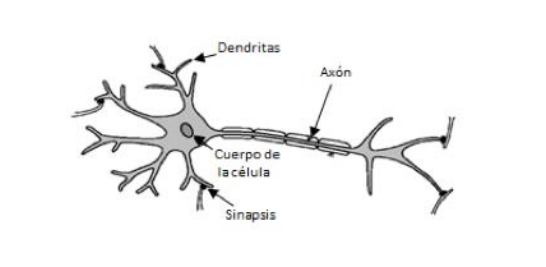
\includegraphics[scale=0.70]{./neuroma_humana.png}
    \caption{Componentes de una neurona.}
    \label{fig:componentes}
  \end{center}
\end{figure}


\subsection{Capas de la neurona artificial}
\textbf{\textit{Desde un punto de vista funcional}}, las neuronas constituyen procesadores de información sencillos, integrados por:
Un canal de recepción de información, las dendritas, que reciben señales de entrada (inputs) procedentes de otras células (interneuronas) o del exterior (neuronas receptoras o sensoras, como los conos y bastones de la retina)\cite{sanchez2015maquinas}.

\textbf{\textit{Un órgano de cómputo}}, el soma, que combina e integra los inputs recibidos (generalmente a través de funcionales no lineales), emitiendo señales de salida en forma de estímulos nerviosos\cite{sanchez2015maquinas}.

\textbf{\textit{Un canal de salida}}, el axón, que envía la salida generada por el soma a
otras neuronas o bien, en el caso de las neuronas motoras, directamente al
músculo. Para transmitir la información, el axón se conecta a través de sus ramificaciones a las dendritas de otras neuronas, que reciben las señales y las combinan para producir nuevas salidas. Una neurona del córtex cerebral recibe información, por término medio, de unas 10.000 neuronas (convergencia), y envía impulsos a varios cientos de ellas (divergencia)\cite{sanchez2015maquinas}.

\begin{figure}[H]
  \begin{center}
    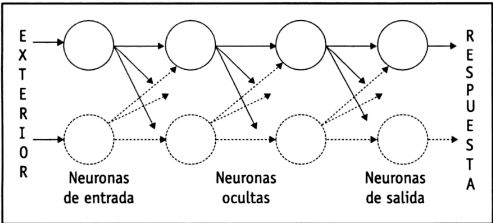
\includegraphics[scale=0.90]{./tipo_neuronas.png}
    \caption{Tipos de neuronas artificiales\cite{lopez2008redes}.}
    \label{fig:tipo}
  \end{center}
\end{figure}

Caracteristicas de tres tipos de neuronas artificiales:
unidades de entrada, de salida y unidades ocultas(Figura~\ref{fig:tipo})\cite{lopez2008redes}.

\begin{itemize}
\item  Las neuronas de entrada reciben señales desde el entorno, provenientes de sensores o de otros sectores del sistema (como archivos de almacenamiento de patrones de aprendizaje).

\item Las neuronas de salida envían su señal directamente fuera del sistema una vez finalizado el tratamiento de la información (salidas de la red).

\item Las neuronas ocultas reciben estímulos y emiten salidas dentro del sistema, sin mantener contacto alguno con el exterior. En ellas se lleva a cabo el procesamiento básico de la información, estableciendo la representación
interna de ésta.
\end{itemize}

\subsection{Modelo de redes neuronales artificiales}

Las redes neuronales artificiales son motivadas por ciertas cualidades de su modelo real, por lo cual el
desafio es producir un modelo que tenga \cite{nacelle2009redes}:
\begin{itemize}
\item  Una estructura de procesamiento distribuida y paralela (opuestamente al CPU de una comutadora).

La arquitectura de las ANN parte de la organización de los sistemas de procesado en paralelo, es decir, sistemas en los que distintos procesadores están interconectados. No
obstante los procesadores son unidades procesadoras simples, diseñadas para la suma de muchas entradas y con un ajuste automático de las conexiones ponderadas. 
\item Alto grado de conexion entre las unidades basicas.
\item Conexiones modificables en funcion de la experiencia.
\item Un proceso de aprendizaje constante y de ser posible uno no supervisado
\item Aprendisaje basado en informacion local.
\item Robustez en la performance si algunas unidades son removidas.

\end{itemize}

\subsection{Arquitectura de una red neuronal}
La topotogia o arquitectura hace referencia a la organización y disposición de las neuronas en la red formando capas de procesadores interconectados entre sí a través de sinapsis unidireccionales. La arquitectura de una RNA depende de cuatro parámetros principales \cite{lopez2008redes}: 

\begin{itemize}
\item el número de capas,
\item el número de neuronas por capa,
\item el grado de conectividad entre las neuronas y 
\item el tipo de conexiones neuronales. 
\end{itemize}


\vspace{1\baselineskip}
Las arquitecturas neuronales pueden clasificarse atendiendo a distintos criterios \cite{lopez2008redes}:

\begin{itemize}
\item Según su estructura en capas
\begin{itemize}
  \item Redes monocapa, compuestas por una única capa de neuronas, entre las que se establecen conexiones laterales y, en ocasiones, autorrecurrentes. Este tipo de redes suele utilizarse para la resolución de problemas de autoasociación y clusterización.

  \item Redes multicapa (layered networks), cuyas neuronas se organizan en varias capas (de entrada, oculta(s) y de salida). La capa a la que pertenece la neurona puede distinguirse mediante la observación del origen de las señales que recibe y el destino de la señal que genera.
\end{itemize}

\item Según el flujo de datos en la red

\begin{itemize}
  \item Redes unidireccionales o de propagación hacia adelante (feedforward), en las que ninguna salida neuronal es entrada de unidades de la misma capa o de capas precedentes. La información circula en un único sentido, desde las neuronas de entrada hacia las neuronas de salida de la red.

  \item Redes de propagación hacia atrás (feedback), en las que las salidas de las neuronas pueden servir de entradas a unidades del mismo nivel (conexiones laterales) o de niveles previos. Las redes de propagación hacia atrás que presentan lazos cerrados se denominan sistemas recurrentes.
\end{itemize}
\end{itemize}

\section{Redes neuronales recurrentes (RNN)}

Las redes neuronales recurrentes tienen caminos de retroalimentación entre todos los elementos que las conforman \cite{montesdeoca2016estudios}. Una sola neurona está entonces conectada a las neuronas posteriores en la siguiente capa, las neuronas pasadas de la capa anterior y a ella misma a través de vectores de pesos variables que sufren alteraciones en cada época con el fin de alcanzar los parámetros o metas de operación.

Las redes neuronales recurrentes (RNNs) son un tipo de modelo de aprendizaje profundo que se utiliza para analizar datos secuenciales, como el procesamiento del lenguaje natural o la predicción de series de tiempo\cite{tomas2023prediccion}.

A diferencia de las redes neuronales artificiales ya vistas, que asumen la independencia entre los datos de entrada, las \gls{rnn} capturan activamente sus dependencias secuenciales y temporales\cite{arana2021redes}.

Las RNN generalmente aumentan la arquitectura de red multicapa convencional con la adición de ciclos que conectan nodos adyacentes o pasos de tiempo.

Estos ciclos constituyen la memoria interna de la red que se utiliza para evaluar las propiedades del dato actual con respecto a los datos del pasado inmediato.

Las redes neuronales recurrentes son más eficaces para resolver problemas con no­linealidades temporales significativas. Son especialmente útiles en aplicaciones tales
como el reconocimiento de patrones secuenciales, cambiantes en el tiempo, ya que las capacidades de predicción y mapeo de las RNN así lo permiten\cite{montesdeoca2016estudios}..

Sin embargo, la capacidad de las RNNs para manejar datos a largo plazo se ve comprometida por el problema del gradiente que desaparece, que ocurre cuando el gradiente se hace cada vez más pequeño a medida que se propaga hacia atrás en la red\cite{tomas2023prediccion}.


Para  superar  este  problema,  Hochreiter \& Schmidhuber,  propusieron  la  memoria  a  corto  y  largo  plazo  (LSTM),  una  variante  de  las  RNNs  que  ha  demostrado  ser efectiva para el procesamiento de datos secuenciales a largo plazo\cite{tomas2023prediccion}.


\subsection{Arquitectura básica de una RNN}
Arquitectura básica de una RNN. Una característica importante es la inclusión de retrasos ($z^{-1}$) a la salida de las neuronas en las capas intermedias; las salidas parciales $S_{mn}(t + 1)$ se convierten en valores $S_{mn}(t)$, un instante de tiempo anterior, y así se retroalimenta a todos los componentes de la red, guardando información de instantes de tiempo anteriores \cite{montesdeoca2016estudios}.Se puede apreciar cómo todos los nodos están interconectados entre sí, estableciendo conexiones tanto directas como mediante retardos temporales con los nodos precedentes en cada capa, lo que permite la incorporación de memorias temporales.

\begin{figure}[H]
  \begin{center}
    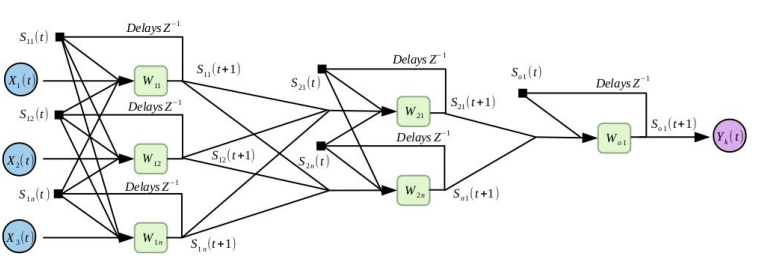
\includegraphics[scale=0.70]{./redes_recurrentes.png}
    \caption{La arquitectura básica de una RNN}
    \label{fig:red_recurreente}
  \end{center}
\end{figure}

\newacronym{lstm}{LSTM}{Redes de Memoria Corta y Larga}
\glsreset{lstm} % reinicia el banderín del primer uso
 
\subsection{Redes de Memoria Corta y Larga  LSTM}

Las redes de “larga memoria de corto plazo”(\gls{lstm}), propuestas por Hochreiter y Schmidhuber. Es una de las arquitecturas de aprendizaje profundo más avanzadas y exitosas para predicción de series temporales, reconocimiento de escritura y análisis de discurso\cite{fernandez2021estimacion}.

El modelo matemático de LSTM se define como una función no lineal que transforma la entrada actual, el estado anterior y la memoria a largo plazo en una salida y un estado actualizado.

El cálculo de esta función implica la  operación  de  multiplicación  de  matrices  y  la  aplicación  de  funciones  de  activación,  como la función sigmoide o la tangente hiperbólica\cite{tomas2023prediccion}.

El objetivo es mejorar la memoria de la RNN de los eventos pasados entrenándola para que recuerde lo importante y olvide el resto. Para ello, las LSTM procesan dos versiones del pasado\cite{arana2021redes}.
\subsection{Los pesos sinápticos}
A una neurona artificial se le asigna un peso sináptico a las entradas que provienen desde otras neuronas. Este procedimiento es similar al que se realiza en una neurona de un ser humano, a lo que normalmente en la medicina se le conoce como sinapsis. El peso sináptico entonces es un valor numérico y que puede ir cambiando durante la fase de entrenamiento\cite{acevedo2017principios}. Este peso hace que la red neural tengo una utilidad y es allí donde se almacena la información.

En una red de neuronas existe un peso o fuerza sináptica que va a ser un valor numérico que pondera las señales que se reciben por sus entradas. Este peso será un valor que determina la fuerza de conexión entre 2 neuronas. Cuando se evalúa una neurona se debe calcular el conjunto de todas las fuerzas o valores (denominado NET) que se reciben por sus entradas. Una vez calculado el valor conjunto de todas las entradas se aplica una función de activación (FA) que determinará el valor del estado interno de la neurona y que será lo que se transmita a su salida\cite{pose2009introduccion}.

\subsection{Perceptron}
En 1957, Frank Rosenblatt publicó el mayor trabajo de investigación en computación neuronal realizado hasta esas fechas. Su trabajo consistía en el desarrollo de un
elemento llamado “Perceptron” \cite{olabe1998redes}.

\vspace{1\baselineskip}
El perceptron es un sistema clasificador de patrones que puede identificar patrones geométricos y abstractos. El primer perceptron era capaz de aprender algo y era robusto, de forma que su comportamiento variaba sólo si resultaban dañados los componentes del sistema. 
Además presentaba la característica de ser flexible y comportarse correctamente después de que algunas celdas fueran destruidas.
El perceptron fue originalmente diseñado para el reconocimiento óptico de patrones.
Una rejilla de 400 fotocélulas, correspondientes a las neuronas de la retina sensibles a la luz, recibe el estímulo óptico. Estas fotocélulas están conectadas a elementos asociativos que recogen los impulsos eléctricos emitidos desde las fotocélulas. Las
conexiones entre los elementos asociativos y las fotocélulas se realizan de forma aleatoria.
Si las células presentan un valor de entrada superior a un umbral predeterminado entonces el elemento asociativo produce una salida\cite{olabe1998redes}.

\begin{figure}[H]
  \begin{center}
    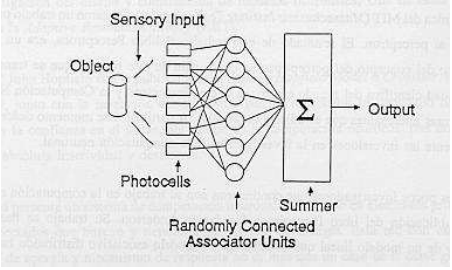
\includegraphics[scale=0.90]{./perceptron.png}
    \caption{Aplicación de la Red Perceptron}
    \label{fig:perceptron}
  \end{center}
\end{figure}

\subsection{Perceptrón multica}
Una Perceptrón multicapa (MLP) puede ser interpretada como una extensión del algoritmo de regresión logística donde primero la entrada es transformada utilizando una transformación no lineal\cite{de2014aprendizaje}. El propósito de esta transformación es proyectar los datos de entrada a un espacio donde sean linealmente separables.
Esta capa intermedia es conocida como capa oculta y es característica de una MLP poseer dos o mas de ellas. Una capa oculta única es suficiente para hacer de una MLP un aproximador universal.

\section{Series de Tiempo}
Las series de tiempo, son datos estadísticos que se recopilan, observan o registran en intervalos de tiempo regulares (diario, semanal, semestral, anual, entre otros)\cite{herrera2020prediccion}. 

Conviene recalcar que una serie de tiempo es un conjunto ordenado de valores, no una función, y que no debe ser tratada como tal\cite{nava2015procesamiento}.

\newacronym{rnn}{RNN}{Redes neuronales recurrentes}
\glsreset{rnn} % reinicia el banderín del primer uso



\section{Antecedentes}
En el proyecto titulado \textbf{\textit{“Desarrollo de un Sistema de Control de Inventario para la Gestión de Compras de Materia Prima en el Rubro de Restaurantes”}} \cite{condorena2017desarrollo}. 

Este antecedente presenta un estudio de caso relevante en el ámbito de la gestión de inventario y compras en la industria de restaurantes. Se describe cómo se implementó con éxito un sistema de control de inventario utilizando el modelo de desarrollo de ciclo de vida en cascada. El objetivo principal de esta implementación fue mejorar la gestión de los procesos de almacén y reducir los tiempos innecesarios en la entrega de productos a los clientes. El sistema se dividió en módulos específicos, centrándose en el almacén y ofreciendo diversas funcionalidades para la gestión eficiente del restaurante. Los resultados obtenidos demuestran una modernización efectiva de los procesos de la empresa en el rubro de restaurantes, con mejoras significativas en la gestión y una reducción sustancial de los tiempos de almacenamiento. Este antecedente sirve como base para la presente tesis, que se enfoca en el desarrollo de un sistema de compra inteligente basado en el historial de ventas, aprovechando la experiencia exitosa de la implementación previa para impulsar la eficiencia operativa en la industria de alimentos
% Se empleó el modelo de desarrollo de ciclo de vida en cascada para desarrollar un sistema de control de inventario para un restaurante con el objetivo de mejorar la gestión de los procesos de almacén y reducir los tiempos innecesarios en la entrega del producto final al cliente. El sistema se divide en los módulos de almacén, que ofrecen diferentes funcionalidades para el desarrollo y gestión del restaurante. Como resultado, el sistema moderniza los procesos de la empresa en el rubro de restaurantes, aportando una mejora significativa en la gestión y reducción de tiempos innecesarios en el almacén. 



\vspace{1\baselineskip}
En el trabajo titulado \textbf{\textit{ “Optimización de la cadena de abastecimiento a través de un sistema inteligente de pronósticos de demanda y gestión de inventario multiproducto”}} \cite{pacheco2015rediseno}. 

El objetivo principal del proyecto fue desarrollar una aplicación web que automatizara parcialmente las actividades del área de compras y mejorara la cadena de abastecimiento mediante un sistema inteligente de pronósticos de demanda y gestión de inventario multiproducto. 
Este antecedente se presenta como una sólida prueba de concepto para la implementación de sistemas inteligentes de gestión de compras basados en pronósticos de demanda en la industria gastronómica, lo que respalda y valida la relevancia de la presente tesis sobre un sistema de compra inteligente basado en historial de ventas.


% Se propone una metodo de seis pasos para optimizar el área de compras y reducir costos en dos empresas del sector gastronómico: EV e IS. El objetivo general del proyecto es construir una aplicación web que semiautomatice las actividades del área de compras y optimice la cadena de abastecimiento a través de un sistema inteligente de pronósticos de demanda y gestión de inventario multiproducto. Se logró una mejora en los errores de pronóstico de 22 \%   en 2 meses, 16 \% en 8 meses y 10 \% en 12 meses. Los resultados económicos indican un VAN de \$61 millones en 3 años y una TIR de 280 \%.

\vspace{1\baselineskip}
En el artículo titulado  \textbf{\textit{“Plan de gestión para la creación de una plataforma tecnológica en un establecimiento gastronómico” }}\cite{sanchez2018sistemas}. Los autores proponen la implementación de una plataforma tecnológica en un restaurante, combinando metodologías de gestión tradicionales y ágiles. El objetivo es mejorar la eficiencia y eficacia en las tareas de atención, supervisión, control y administración del establecimiento gastronómico. La metodología SCRUM se utilizará para la gestión del desarrollo, utilizando las estimaciones previas como métricas de evolución para identificar posibles retrasos e inconvenientes. El plan de proyecto estima los alcances, costos y duración de las tareas de desarrollo, definiendo planes de gestión de calidad y mitigación de riesgos. La combinación de metodologías utilizada busca generar una solución eficiente para la administración del desarrollo de la plataforma tecnológica. 

% \vspace{1\baselineskip}
% El plan de proyecto detalla estimaciones de alcance, costos y duración de las actividades de desarrollo, y establece planes para la gestión de calidad y mitigación de riesgos. La combinación de enfoques metodológicos adoptada en este proyecto busca ofrecer una solución eficaz para la administración y desarrollo exitoso de la plataforma tecnológica en el contexto de la industria gastronómica.

\vspace{1\baselineskip}
El artículo \textbf{\textit{ “Reducing Food Waste in the Food Industry with Deep Learning” }}\cite{afanador2022diseno}. 

El autor, Esteban David Romero Pérez, se centra en la importante tarea de ayudar a la industria alimentaria a anticipar con precisión la demanda de sus productos y, por lo tanto, reducir los excedentes no vendidos, lo que está alineado con el Objetivo de Desarrollo Sostenible número 12 de las Naciones Unidas. Los resultados obtenidos en este estudio demuestran de manera convincente que la aplicación de Deep Learning puede conducir a una disminución sustancial en la cantidad de alimentos desperdiciados en la industria alimentaria, contribuyendo significativamente a un futuro más sostenible y eficiente en el uso de recursos. Este antecedente resalta la relevancia de la tecnología de aprendizaje profundo en la optimización de procesos en la industria alimentaria, lo que puede ser de gran utilidad para el enfoque de la presente tesis.

% Escrito por Esteban David Romero Pérez aborda el objetivo de reducir el desperdicio de alimentos en la industria alimentaria utilizando la tecnología de Deep Learning. El enfoque del artículo es ayudar a la industria alimentaria a predecir la cantidad de platos que se pueden vender en una semana específica, lo que ayudará a minimizar los desperdicios de alimentos y cumplir con el objetivo número 12 de la Organización de las Naciones Unidas para el desarrollo sostenible. Los resultados obtenidos muestran una disminución significativa en la cantidad de alimentos desperdiciados en la industria alimentaria, lo que contribuye a un futuro más sostenible.

% \vspace{1\baselineskip}


\vspace{1\baselineskip}
En un estudio llevado a cabo en Móstoles, España titulado \textbf{\textit{“Un análisis de sentimiento en Twitter con Machine Learning: Identificando el sentimiento sobre las ofertas de \#BlackFriday” }}\cite{saura2018analisis}. Se estableció una conexión con la API de Twitter para recopilar un total de 2204 tweets relacionados con los comentarios e interacciones de los usuarios acerca de las ofertas proporcionadas por empresas en la muestra. Posteriormente, se aplicó un algoritmo de análisis de sentimiento desarrollado en Python utilizando la biblioteca MonkeyLearn para categorizar estos tweets en positivos y negativos. Se centró en evaluar la percepción de los usuarios sobre las ofertas del Black Friday a través del análisis automatizado de los comentarios en Twitter.

\vspace{1\baselineskip}
Tesis\textbf{\textit{“Prediccion de la demanda usando modelos de machine Learning” }}\cite{hincapie2021prediccion} Para aquellas empresas dedicadas a la venta en retail o venta directa donde su portafolio de productos es muy amplio, la planeación de la demanda se convierte en un área determinante para la correcta administración del flujo de caja, rentabilidad y efectividad en ventas por varias razones: la primera de ellas es la gestión de compra de insumos por medio de negociación de precio por volumen con sus proveedores; el control de inventario donde se cuide un equilibrio entre uso efectivo del espacio de almacenamiento y reducción de obsolescencia contra la disponibilidad para distribución y por último en la venta efectiva respetando las estacionalidades, tendencias del mercado y satisfacción del cliente.

% \vspace{1\baselineskip}
% La planeación de la demanda en empresas minoristas con una amplia gama de productos es crucial para gestionar la compra de insumos, controlar el inventario y maximizar las ventas. Se emplean modelos de regresión, como Random Forest Regressor y H2O AutoML, junto con análisis de tipicidad, para predecir con precisión las unidades de productos a vender y optimizar la gestión de categorías, lo que mejora la eficiencia y rentabilidad.


\vspace{1\baselineskip}
Trabajo final de grado tiulado \textbf{\textit{“Estudios de predicción en series temporales de datos meteorológicos utilizando redes neuronales recurrentes” }}\cite{montesdeoca2016estudios}
En los últimos años, en el campo de las energías renovables, la energía eólica ha sido una de las que mas se ha desarrollado e invertido. La importancia de las predicciones de viento radica en la ayuda que aportan para planificar y anticiparse a los valores futuros que afectarán al sistema, ayudando a gestionar la adquisición de los recursos necesarios con antelación suficiente. Recientemente se han desarrollado nuevas arquitecturas de redes recurrentes que resultan muy prometedoras para realizar predicción. En este trabajo se probará y experimentará con dichas arquitecturas para realizar distintas predicciones de la velocidad del viento en un horizonte de corto y muy corto plazo a partir de datos de series temporales de viento.

